% Lecture file created by newnote
% Class: Models of Theoretical Physics
% Professor: Azaele Sandro
% Date: 2025-10-17
\lecture{10}{Introduction to Stochastic Differential Equations}{2025-10-17}
\pagelayout{margin}
% --- Start writing here ---

\section{Introduction to Stochastic Differential Equations}
We have already seen a very simple example of SDE in eq. (4) and (5) where $x(t)=x_{0}+\mu t+\sigma B(t)$ or $d x=\mu d t+\sigma d B(t)$. This was also easy to integrate numerically. Usually an ODE has the form
\begin{DispWithArrows}[tag=25]
    \frac{d x}{d t}=f(x, t)
\end{DispWithArrows}
Can we write an SDE in this usual form? Let's try. We get from
\begin{DispWithArrows}
    \frac{d x}{d t}=\mu+\sigma \dot{B}(t)
\end{DispWithArrows}
What is $\dot{B}$? Actually it does not exist because we have seen that Brownian motion is nowhere differentiable. However, $\Delta B=B(t+\Delta t)-B(t)$ is well defined, so mathematicians prefer the notation $d x=\mu d t+\sigma d B$. However, we can give a meaning to the "pseudo notation" $\dot{B}$. We first discretize and then take the limit as $\Delta t \rightarrow 0$; so we define for a finite $\Delta t \quad \xi_{\Delta, i}=\frac{\Delta B_{i}}{\Delta t}, \Delta B_{i} \equiv B\left(t_{i}+\Delta t\right)-B\left(t_{i}\right)$. As we know, $\Delta B_{i}$ does not depend on $t_{i}$, but this notation is useful in the following. Of course, $\left\langle\xi_{\Delta, i}\right\rangle=0$. In order to understand what $\left\langle\xi_{\Delta, i} \xi_{\Delta, j}\right\rangle$ is, let's take a test function $g(t)$ and calculate at $g_{i} \equiv g\left(t_{i}\right)$ the following
\begin{DispWithArrows}
    \sum_{j} g_{j}\left\langle\xi_{\Delta, i} \xi_{\Delta, j}\right\rangle \Delta t=\sum_{j} g_{j}\left\langle\frac{\Delta B_{i}}{\Delta t} \frac{\Delta B_{j}}{\Delta t}\right\rangle \Delta t=\sum_{j} g_{j} \frac{\left\langle\Delta B_{i} \Delta B_{j}\right\rangle}{\Delta t} = \sum_{j} g_{j} \frac{\delta_{i j} \Delta t}{\Delta t}=g_{i}
\end{DispWithArrows}
N.B: $\left\langle\Delta B_{i} \Delta B_{j}\right\rangle=\delta_{i j} \Delta t$

If we now take the continuum limit $\Delta t \rightarrow 0$, and "$\\lim _{\Delta t \rightarrow 0} \xi_{\Delta, i} \equiv \xi(t)$" we get
\begin{DispWithArrows}
    \int g\left(t^{\prime}\right)\left\langle\xi(t) \xi\left(t^{\prime}\right)\right\rangle d t^{\prime}=g(t)
\end{DispWithArrows}
Which therefore means that $\left\langle\xi(t) \xi\left(t^{\prime}\right)\right\rangle=\delta\left(t-t^{\prime}\right)$ and $\langle\xi(t)\rangle=0$. This is called Gaussian white (or $\delta$-correlated) noise; with this we can then write the SDE in eq. (4) as
\begin{DispWithArrows}[tag=26]
    \begin{gathered}
    \dot{x}(t)=\mu+\sigma \xi(t) \\    \langle\xi\rangle=0 \quad\left\langle\xi(t) \xi\left(t^{\prime}\right)\right\rangle=\delta\left(t-t^{\prime}\right)\end{gathered} \quad \text { is equivalent to } \quad d x=\mu d t+\sigma d B(t)
\end{DispWithArrows}
$B(t)$ is a standard B.M. $\langle B(t)\rangle=0, \langle B(t) B(s)\rangle=t \wedge s$

The first one is a notation which physicists like the most, whereas mathematicians prefer $d x=\mu d t+d B$, you can find both in the literature.

\subsection*{What is a solution?}
If we start from a deterministic eq like
\begin{DispWithArrows}
    d x=f(x, t) d t
\end{DispWithArrows}
there are many ways to introduce noise. We could define a stoch. process by saying that $d x=\tilde{f}(x, t, d B) d t$ where $\tilde{f}$ is a generic non-linear smooth function. However this definition does not work in general and it is very difficult to define appropriately what that exactly means and to able to find solutions.
The approach that works in many situations, even in higher dimensions under general assumptions is to introduce the noise (better, Brownian motion) in an additive way. This means that we can develop a good deal of theory for SDEs of the form
\begin{DispWithArrows}[tag=27]
    d x=\mu(x, t) d t+\sigma d B(t) \quad(\sigma>0)
\end{DispWithArrows}
where $\mu$ is a smooth function of $x, t$. This eq. can be also justified on physical grounds as we will see in the following (if $x(t)$ is the position of a large particle in a fluid, $\sigma dB$ can represent the effect of all other small fluid particles at temperature $T$, and $\sigma=\sigma(T)$, which continuously kick the large one. All kicks produce the erratic movement of the big suspended particle).
Eq. (27) is called Langevin equation with additive noise.
However, even simple equations such as this one
\begin{DispWithArrows}
    d x=-\mu x d t+\sigma d B
\end{DispWithArrows}
can hide pitfalls. For instance, $\langle d x\rangle=-\mu\langle x\rangle d t$, so $\frac{d\langle x\rangle}{d t}=-\mu\langle x\rangle$ hence $\langle x(t)\rangle=x_{0} e^{-\mu t}$. But what about fluctuations?

We need to calculate $\left\langle x^{2}\right\rangle$. Let's proceed naively with ordinary calculus: $\frac{d x^{2}}{d t}=2 x \frac{d x}{d t}$, so $2 x d x=-2 \mu x^{2} d t+2\sigma x d B$ and $d\left\langle x^{2}\right\rangle=2\langle x d x\rangle=-2 \mu\left\langle x^{2}\right\rangle d t+2 \sigma\langle x d B\rangle=-2 \mu\left\langle x^{2}\right\rangle d t$
then $\frac{d\left\langle x^{2}\right\rangle}{d t}=-2 \mu\left\langle x^{2}\right\rangle \Rightarrow\left\langle x^{2}\right\rangle=x_{0}^{2} e^{-2 \mu t}$. But then
\begin{DispWithArrows}
    \sqrt{\left\langle x^{2}\right\rangle}=x_{0} e^{-\mu t}=\langle x\rangle \Rightarrow \operatorname{Var}[x(t)]=0!
\end{DispWithArrows}
So there are no fluctuations even if we add the noise! Either ordinary calculus cannot be used or $\langle x d B\rangle \neq 0$. This is a consequence of the non-differentiability of $B$.

We can consider SDEs even more general SDEs than eq.(27) driven by Brownian motion
\begin{DispWithArrows}[tag=28]
    d x=\mu(x, t) d t+\sigma(x, t) d B
\end{DispWithArrows}
This is an SDE with multiplicative noise because $\sigma$ is a function of the state $x$. Eq. (28) needs extra care!

If we have a (strong) solution $x(t)$ of eq. (28) then we can write
\begin{DispWithArrows}[tag=28b]
    x(t)=x(0)+\int_{0}^{t} \mu(x(s), s) d s+\int_{0}^{t} \sigma(x(s), s) d B(s)
\end{DispWithArrows}
A strong solution is some functional $F(t, B(s), s \leq t)$ of the Brownian motion $B(t)$. This becomes the solution of the corresponding ODE as $\sigma=0$.

Warning:
What is the meaning of $\int_{0}^{t} \sigma(x(s), s) d B(s)$? Can this be understood as an ordinary integral? No.

Let's take a very simple example. If the process is simply ($\mu=0$ and $\sigma=B$):
\begin{DispWithArrows}
    d x=B(t) d B(t)
\end{DispWithArrows}
the solution is $X(t)=\int_{0}^{t} B(s) d B(s)$
So we naively expect $E[x(t)]=0$

If we use ordinary calculus then
\begin{DispWithArrows}
    x(t)=\frac{B(t)^{2}}{2}
\end{DispWithArrows}
but then $\mathbb{E}[x(t)]=\frac{t}{2} \neq 0$. What's going on here?
Again, because Brownian motion is very irregular, it gives rise to problems where interpreting solutions or eqs.

Before showing what the nature of the problem is, we have to prove an important property of the Brownian m.

\subsection*{LEMMA: The Brownian motion has finite quadratic variation}
Let's fix $t>0$, take the interval $[0, t]$ and partitions $\mathcal{P}_{n}$ of the interval $\left\{t_{0}=0<t_{1}<t_{2} \cdots<t_{n}=t\right\}$ such that $\left|\mathcal{P}_{n}\right| \equiv \max _{i}\left|t_{i}-t_{i-1}\right| \rightarrow 0$ as $n \rightarrow \infty$. Then
\begin{DispWithArrows}[tag=29]
    \operatorname{ms-lim}_{\substack{n \rightarrow \infty \\ \left|\mathcal{P}_{n}\right| \rightarrow 0}} \sum_{i=0}^{n-1} \underbrace{\left[B\left(t_{i+1}\right)-B\left(t_{i}\right)\right]^{2}}_{\text{quadratic variation}}}=t
\end{DispWithArrows}
Reminder: $\underset{n \rightarrow \infty}{m s-\lim } x_{n}=x$ means $\lim _{n \rightarrow \infty}\left\langle\left(x_{n}-x\right)^{2}\right\rangle=0$ this is the mean square limit and we say that $x_{n}$ converges to $x$ in the mean square.

Proof: Let's define $Q_{n} \equiv \sum_{i=0}^{n-1}\left[B\left(t_{i+1}\right)-B\left(t_{i}\right)\right]^{2}$ and take
\begin{DispWithArrows}
    Q_{n}-t=\sum_{i}\left\{\left[B\left(t_{i+1}\right)-B\left(t_{i}\right)\right]^{2}-\left(t_{i+1}-t_{i}\right)\right\}
\end{DispWithArrows}
Hence we have to evaluate as $n \rightarrow \infty \quad\left(B\left(t_{i}\right) \equiv B_{i}\right)$
\begin{DispWithArrows}[tag=29b]
    \mathbb{E}\left[\left(Q_{n}-t
ight)^{2}\right]=\sum_{i=0}^{n-1} \sum_{j=0}^{n-1} \mathbb{E}\left[\left\{\left(B_{i+1}-B_{i}\right)^{2}-\left(t_{i+1}-t_{i}\right)\right\}\left\{\left(B_{j+1}-B_{j}\right)^{2}-\left(t_{j+1}-t_{j}\right)\right\}\right]
\end{DispWithArrows}
For $i \neq j$
\begin{DispWithArrows}
    \begin{aligned}
    & \mathbb{E}\left[\left\{\left(B_{i+1}-B_{i}\right)^{2}-\left(t_{i+1}-t_{i}\right)\right\}\left\{\left(B_{j+1}-B_{j}\right)^{2}-\left(t_{j+1}-t_{j}\right)\right\}
ight] \\    &= \mathbb{E}\left[\left\{\left(B_{i+1}-B_{i}\right)^{2}-\left(t_{i+1}-t_{i}\right)\right\}\right] \mathbb{E}\left[\left\{\left(B_{j+1}-B_{j}\right)^{2}-\left(t_{j+1}-t_{j}\right)\right\}\right]=0
    \end{aligned}
\end{DispWithArrows}
$\\mathbb{E}\left[\left(B_{i+1}-B_{i}\right)^{2}\right]=t_{i+1}-t_{i}$

Therefore eq. (29b) becomes
\begin{DispWithArrows}
    \begin{aligned}
    \mathbb{E}\left[\left(Q_{n}-t
ight)^{2}\right] & =\sum_{i=0}^{n-1} \mathbb{E}\left[\left\{\left(B_{i+1}-B_{i}\right)^{2}-\left(t_{i+1}-t_{i}\right)\right\}^{2}\right] \\    & =\sum_{i}\left\{\mathbb{E}\left[\left(B_{i+1}-B_{i}\right)^{4}\right]-2 \mathbb{E}\left[\left(B_{i+1}-B_{i}\right)^{2}\right]\left(t_{i+1}-t_{i}\right)+\left(t_{i+1}-t_{i}\right)^{2}\right\} \\    & =\sum_{i}\left\{3\left(t_{i+1}-t_{i}\right)^{2}-2\left(t_{i+1}-t_{i}\right)^{2}+\left(t_{i+1}-t_{i}\right)^{2}\right\} \\    & =2 \sum_{i}\left(t_{i+1}-t_{i}\right)^{2} \leq 2 \max _{i}\left(t_{i+1}-t_{i}\right) \sum_{i}\left(t_{i+1}-t_{i}\right)=2\left|\mathcal{P}_{n}\right| t \rightarrow 0
    \end{aligned}
\end{DispWithArrows}
One can show that the convergence is even stronger, it is almost sure: $\lim _{n} Q_{n}=t$. It is remarkable that, although $Q_{n}$ is random for any finite $n$, its limit is not!

This lemma partly justifies the heuristic idea that
\begin{DispWithArrows}[tag=30]
    |d B| \simeq \sqrt{d t}
\end{DispWithArrows}
which we will use many times in the future.

If we interpret $x(t)=\int_{0}^{t} B(s) d B(s)$ as the limit of Riemann sums as in the ordinary definition of integrals, we have to discretize it and then take the limit. The following theorem will show the nature of the "problem".

\subsection*{Theorem}
Let's take the interval $[0, t](t>0)$ and partitions $\mathcal{P}_{n}$ of the interval $\left\{t_{0}=0<t_{1}<t_{2} \cdots<t_{n}=t\right\}$ such that $\left|\mathcal{P}_{n}\right| \equiv \max _{i}\left|t_{i}-t_{i-1}\right| \rightarrow 0$ as $n \rightarrow \infty$. Also fix $\lambda \in \mathbb{R}, 0 \leq \lambda \leq 1$ and define
\begin{DispWithArrows}
    X_{n} \equiv \sum_{i=0}^{n-1} B\left(\lambda t_{i+1}+(1-\lambda) t_{i}\right)\left[B\left(t_{i+1}\right)-B\left(t_{i}\right)\right]
\end{DispWithArrows}
then
\begin{DispWithArrows}[tag=31]
    \operatorname{ms-lim}_{\substack{n \rightarrow 
 \infty \\ \left|\mathcal{P}_{n}\right| \rightarrow 0}} X_{n}=\frac{[B(t)]^{2}}{2}+\left(\lambda-\frac{1}{2}\right) t
\end{DispWithArrows}
\begin{figure}[H]
    \centering
    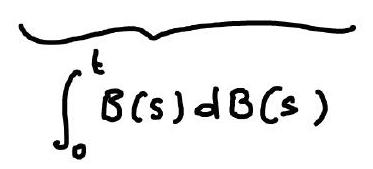
\includegraphics[width=0.5\textwidth]{2025_10_17_a59e220b8a74630d2381g-07}
\end{figure}

\subsection*{COMMENTS:}
We recognize $X_{n}$ as the Riemann sum corresponding to $x(t)$ where we take an arbitrary intermediate point in $\left[t_{i}, t_{i+1}\right]$. In ordinary calculus the integral does not depend on the location of the intermediate point, however in the stochastic integral there is an unavoidable dependence on which point we choose. This is one of the most important features of the stochastic calculus with Brownian motion.
proof:
We introduce a more compact notation: $B_{i}^{\lambda} \equiv B\left(\lambda t_{i+1}+(1-\lambda) t_{i}\right), B\left(t_{i}\right) \equiv B_{i}$. Then $X_{n}=\sum_{i=0}^{n-1} B_{i}^{\lambda}\left(B_{i+1}-B_{i}\right)$.
We use now the identity (with B.m. everything is easier with squares or squared differences):
\begin{DispWithArrows}
    \begin{aligned}
    B_{i}^{\lambda}\left(B_{i+1}-B_{i}\right) & =\left(B_{i}^{\lambda}-B_{i}+B_{i}\right)\left(B_{i+1}-B_{i}^{\lambda}+B_{i}^{\lambda}-B_{i}\right) \\    & =\left(B_{i}^{\lambda}-B_{i}\right)\left(B_{i+1}-B_{i}^{\lambda}\right)+\left(B_{i}^{\lambda}-B_{i}\right)^{2}+B_{i}\left(B_{i+1}-B_{i}^{\lambda}\right)+B_{i}\left(B_{i}^{\lambda}-B_{i}\right) \\    & =\left(B_{i}^{\lambda}-B_{i}\right)\left(B_{i+1}-B_{i}^{\lambda}\right)+\left(B_{i}^{\lambda}-B_{i}\right)^{2}+B_{i} B_{i+1}-B_{i}^{2} \\    & =\underbrace{\left(B_{i}^{\lambda}-B_{i}\right)\left(B_{i+1}-B_{i}^{\lambda}\right)}_{(\text{D})}+\underbrace{\left(B_{i}^{\lambda}-B_{i}\right)^{2}}_{(\text{C})}-\underbrace{\frac{1}{2}\left(B_{i+1}-B_{i}\right)^{2}}_{(\text{B})}+\underbrace{\frac{B_{i+1}^{2}}{2}-\frac{B_{i}^{2}}{2}}_{(A)}
    \end{aligned}
\end{DispWithArrows}
Let's calculate all the terms:
(A) $\sum_{i=0}^{n-1}\left(\frac{B_{i+1}^{2}}{2}-\frac{B_{i}^{2}}{2}\right)=\frac{1}{2}\left(B_{n}^{2}-B_{0}^{2}\right)=\frac{B^{2}(t)}{2}$
(B) $-\frac{1}{2} \sum_{i=0}^{n-1}\left(B_{i+1}-B_{i}\right)^{2} \xrightarrow{\text{ms-limit}} -\frac{t}{2}$ (lemma)
(C) $\sum_{i=0}^{n-1}\left(B_{i}^{\lambda}-B_{i}\right)^{2} \xrightarrow{\text{ms-limit}} \lambda t$ (use the lemma)
(D) We have to show that the term (D) is zero in the ms-limit:
\begin{DispWithArrows}
    \begin{aligned}
    \mathbb{E}\left[\left(\sum_{i=0}^{n-1}\left(B_{i}^{\lambda}-B_{i}\right)\left(B_{i+1}-B_{i}^{\lambda}\right)\right)^{2}\right] & =\sum_{i=0}^{n-1} \mathbb{E}\left[\left(B_{i}^{\lambda}-B_{i}\right)^{2}\right] \mathbb{E}\left[\left(B_{i+1}-B_{i}^{\lambda}\right)^{2}\right] \\    & =\sum_{i=0}^{n-1} \lambda\left(t_{i+1}-t_{i}\right) \cdot(1-\lambda)\left(t_{i+1}-t_{i}\right) \\    & \leq \lambda(1-\lambda) \max _{j}\left(t_{j+1}-t_{j}\right) \sum_{i=0}^{n-1}\left(t_{i+1}-t_{i}\right) \leq \lambda(1-\lambda)\left|\mathcal{P}_{n}\right| t \rightarrow 0 \text { as } n \rightarrow 
 \infty .
    \end{aligned}
\end{DispWithArrows}
The theorem shows that
\begin{DispWithArrows}[tag=32]
    \int_{0}^{t} B(s) d B(s)=\frac{B^{2}(t)}{2}+\left(\lambda-\frac{1}{2}\right) t
\end{DispWithArrows}
so it does depend in general on the intermediate point that we choose. The main choices are:
(I) $\int_{0}^{t} B(s) d B(s)=\frac{B^{2}(t)}{2}-\frac{t}{2} \quad$ Itô integral, $\lambda=0$
(S) $\int_{0}^{t} B(s) d B(s)=\frac{B^{2}(t)}{2} \quad$ Stratonovich integral, $\lambda=\frac{1}{2}$

\subsection*{IMPORTANT COMMENTS:}
(1) Why should we use Itô? Since $t$ represents time and because we do not know what value B will get in the following interval $\left[t_{i}, t_{i+1}\right]$, we prefer to select the known value in the approximation, i.e. $B\left(t_{i}\right)$. This is the choice in (I).

From eq. (32)
\begin{DispWithArrows}
    \mathbb{E}\left[\int_{0}^{t} B(s) d B(s)\right]=0
\end{DispWithArrows}
So (I) has the strange property that that it does not follow ordinary calculus, but it is handy because one can show that $\mathbb{E}[B(t) d B(t)]=\mathbb{E}[B(t)] \mathbb{E}[d B(t)]=0$. In general for Itô integrals:
\begin{DispWithArrows}
    E\left[\int \sigma d B\right]=\int E[\sigma] E[d B]=0
\end{DispWithArrows}
In the following we will always use the Itô prescription when considering SDEs of the form (28).

Notice that if the SDE is with additive noise (eq. (27)) there is no need to introduce any intermediate prescription.
If we use a function $\sigma(x)$, instead of $B(s)$, and we define $\int_{0}^{t} \sigma(x) d B(s)$ as in eq. (28b), in general $\sigma(x)$ will depend on the B.m. $B(s)$ for $s \leq t$ and we do not know at time $t$ its future value at times $\tau>t$. We don't want $\sigma$ to depend on $B(\tau)-B(s), \forall \tau>s$. All these functions $\sigma(x)$, which depend only on the information available up to time $t$ (so they are indep. of $B(\tau)-B(s), \forall \tau>s$), are called non-anticipating functions. We will always use these functions.
If $\sigma$ is non-anticipating, the Itô stochastic integral ($\lambda=0$) of the function $\sigma(x)$ is defined as
\begin{DispWithArrows}
    \int_{0}^{t} \sigma(s) d B(s)=\lim _{n \rightarrow 
 \infty} \left(\sum_{i=0}^{n-1} \sigma\left(t_{i}\right)\left[B\left(t_{i+1}\right)-B\left(t_{i}\right)\right]\right)
\end{DispWithArrows}
One can also show that ($\sigma$ non-anticipating)
\begin{DispWithArrows}
    \left\langle\left(\int_{0}^{t} \sigma(s) d B(s)\right)^{2}\right\rangle=\int_{0}^{t} d s \left\langle\sigma(s)^{2}\right\rangle
\end{DispWithArrows}
(See Gardiner p. 84): $\operatorname{ms-lim} \sum_{i=0}^{n-1} \sigma_{i}^{2}\left(B_{i+1}-B_{i}\right)^{2}=\int_{0}^{t} d s \sigma(s)^2$
(2) The advantage with the Stratonovich choice ($\lambda=\frac{1}{2}$) is that one can use ordinary calculus, but in this case
\begin{DispWithArrows}
    \mathbb{E}\left[\int_{0}^{t} B(s) d B(s)\right]=\frac{t}{2}
\end{DispWithArrows}
So the B.m. is correlated to the following times.

The dependence on the intermediate point is clear even when calculating the expected value $\mathbb{E}\left[\int_{0}^{t} B(s) d B(s)\right]$.
The discretization gives ($t_{0}=0, t_{n}=t$)
\begin{DispWithArrows}
    \begin{aligned}
    & \mathbb{E}\left[\sum_{i=0}^{n-1} B\left(t_{i}+\lambda\left(t_{i+1}-t_{i}\right)\right)\left(B\left(t_{i+1}\right)-B\left(t_{i}\right)\right)\right]=
 \\    = & \sum_{i} \mathbb{E}\left[B\left(t_{i}+\lambda\left(t_{i+1}-t_{i}\right)\right) B\left(t_{i+1}\right)\right]-\sum_{i}\mathbb{E}\left[B\left(t_{i}+\lambda\left(t_{i+1}-t_{i}\right)\right) B\left(t_{i}\right)\right] \\    = & \sum_{i=0}^{n-1} \left(t_{i}+\lambda\left(t_{i+1}-t_{i}\right)-t_{i}\right)=\lambda t
    \end{aligned}
\end{DispWithArrows}
Exercise: Assume that the stochastic process $g(t)$ depends on the B.m. $B(s)$ for any $s<t$, so $g$ is non-anticipating. Show that $\mathbb{E}\left[\left(\int_{0}^{t} g(s) d B(s)\right)^{2}\right]=\mathbb{E}\left[\int_{0}^{t} g^{2}(s) d s\right]$ if we use the Itô convention.
Hint: use the discretization $\sum_{i=0}^{n-1} g\left(t_{i}\right)\left(B\left(t_{i+1}\right)-B\left(t_{i}\right)\right)$ and, after all the calculations, take the limit $n \rightarrow 
 \infty$.

\subsection*{Itô Calculus}
We have seen that the Brownian motion may lead to a change in the usual calculus. In the following we only show what are the new differentiation rules when using the Itô prescription and the finding that $\Delta B \simeq \sqrt{\Delta t}$
Let's assume that $u(B(t), t)$, then
\begin{DispWithArrows}
    \begin{aligned}
    \Delta u & =u(B(t+\Delta t), t+\Delta t)-u(B(t), t) \stackrel{\downarrow}{=} \frac{\partial u}{\partial t} \Delta t+\frac{\partial u}{\partial B} \Delta B+\frac{1}{2} \frac{\partial^{2} u}{\partial B^{2}} \Delta B^{2}+\text { h.o.t. } \\    & =\left(\frac{\partial u}{\partial t}+\frac{1}{2} \frac{\partial^{2} u}{\partial B^{2}}\right) \Delta t+\frac{\partial u}{\partial B} \Delta B \quad \leftarrow \text { " } \Delta B^{2}=\Delta t \text " \\    & =\left(\frac{\partial u}{\partial t}+\frac{1}{2} \frac{\partial^{2} u}{\partial B^{2}}\right) \Delta t+\frac{\partial u}{\partial B} \Delta B
    \end{aligned}
\end{DispWithArrows}
this term is not present in ordinary calculus and is due to the fact that $|
 \Delta B| \simeq \sqrt{\Delta t}$

The Itô differential rule is
\begin{DispWithArrows}[tag=34]
    d u=\left(\frac{\partial u}{\partial t}+\frac{1}{2} \frac{\partial^{2} u}{\partial B^{2}}\right) d t+\frac{\partial u}{\partial B} d B
\end{DispWithArrows}
Of course, if $u$ does not depend on $t$, $d u=\frac{1}{2} \frac{\partial^{2} u}{\partial B^{2}} d t+\frac{\partial u}{\partial B} d B$.
Example: $u(B)=B^{2}$, then $d B^{2}=d t+2 B d B$. If we then integrate both sides $\int_{t_{1}}^{t_{2}} d\left(B^{2}\right)=B^{2}\left(t_{2}\right)-B^{2}\left(t_{1}\right)=t_{2}-t_{1}+2 \int_{t_{1}}^{t_{2}} B(s) d B(s)$ we get
\begin{DispWithArrows}
    \int_{t_{1}}^{t_{2}} B(s) d B(s)=\frac{B^{2}\left(t_{2}\right)-B^{2}\left(t_{1}\right)}{2}-\frac{t_{2}-t_{1}}{2}
\end{DispWithArrows}
which is in agreement with eq. (I)

Exercise: 1) Calculate the Itô differential for $B_{t}^{n}$ and show that $d B_{t}^{n}=n B_{t}^{n-1} d B_{t}+\frac{n(n-1)}{2} B_{t}^{n-2} d t$ and $\int_{0}^{t} B^{n} d B=\frac{B_{t}^{n+1}}{n+1}-\frac{n}{2} \int_{0}^{t} B(s)^{n-1} d s$
2) By using the Itô differential of $Y(B, t)=e^{\lambda B(t)-\frac{\lambda^{2}}{2} t}$ and that $B(0)=0$, show that $Y(t)=Y(B, t)$ solves the Itô SDE
\begin{DispWithArrows}
    \left\{
    \begin{aligned}
    & d Y(t) \quad=\lambda Y(t) d B(t) \\    & Y(0) \quad=1
    \end{aligned}\right.
\end{DispWithArrows}
Show that $\langle Y(t)\rangle=1 \quad \forall t \geqslant 0$ and $P(y, t)=\frac{e^{-\frac{\left(\ln y+\frac{\lambda^{2} t}{2}\right)^{2}}{2 \lambda^{2} t}}}{\sqrt{2 \pi \lambda^{2} t}} y$. This is called log-normal distribution.

\subsection*{Itô's chain rule (Itô's formula)}
Suppose that $X(t)$ is a stoch. process which satisfies the SDE
\begin{DispWithArrows}
    d x(t)=\mu(x, t) d t+\sigma(x, t) d B(t)
\end{DispWithArrows}
where the SDE is interpreted with the Itô prescription; then if $u(x, t) \in C_{t}^{1}, \in C_{x}^{2}$ then the stochastic process $u$ satisfies the SDE:
\begin{DispWithArrows}[tag=35]
    d u=\left(\frac{\partial u}{\partial t}+\frac{\partial u}{\partial x} \mu+\frac{1}{2} \frac{\partial^{2} u}{\partial x^{2}} \sigma^{2}\right) d t+\frac{\partial u}{\partial x} \sigma d B
\end{DispWithArrows}
Indeed, we use the simple rules: $d t d B=O\left(d t^{3 / 2}\right), d B^{2}=d t$
\begin{DispWithArrows}
    d u=\frac{\partial u}{\partial t} d t+\frac{\partial u}{\partial x} d x+\frac{1}{2} \frac{\partial^{2} u}{\partial x^{2}} d x^{2}+\text { h.o.t. } \\    \text { however } d x^{2}=(\mu d t+\sigma d B)^{2}=\mu^{2} d t^{2}+2 \mu \sigma d t d B+\sigma^{2} d B^{2}=\sigma^{2} d t
\end{DispWithArrows}
then
\begin{DispWithArrows}
    \begin{aligned}
    d u & =\frac{\partial u}{\partial t} d t+\frac{\partial u}{\partial x}(\mu d t+\sigma d B)+\frac{1}{2} \frac{\partial^{2} u}{\partial x^{2}} \sigma^{2} d t \\    & =\left(\frac{\partial u}{\partial t}+\frac{\partial u}{\partial x} \mu+\frac{1}{2} \frac{\partial^{2} u}{\partial x^{2}} \sigma^{2}\right) d t+\frac{\partial u}{\partial x} \sigma d B \text { as in (35) }
    \end{aligned}
\end{DispWithArrows}
Exercise: 1) The stoch. proc. $x(t)$ satisfies the Itô SDE (This process is called geometric Brownian motion).
\begin{DispWithArrows}
    \left\{
    \begin{array}{l}
     d x=\frac{x}{2} d t+x d B \\    x(0)=1
    \end{array}\right.
\end{DispWithArrows}
Show that the process $y=\ln x$ satisfies the Itô SDE
\begin{DispWithArrows}
    \left\{
    \begin{array}{l}
     d y=d B \\    y(0)=0
    \end{array}\right.
\end{DispWithArrows}
and therefore the solution of the original SDE is $x(t)=e^{B(t)}$.
2) Itô formula for 2 variables:

Assume that the two processes $x(t)$ and $y(t)$ satisfy the two Itô SDEs $d x=\mu_{x} d t+\sigma_{x} d B$ and $d y=\mu_{y} d t+\sigma_{y} d B$. By using the Itô rules, show that if $u(x, y) \in C^{2}(x, y)$ then
$d u=\left(\frac{\partial u}{\partial x} \mu_{x}+\frac{\partial u}{\partial y} \mu_{y}+\frac{1}{2} \frac{\partial^{2} u}{\partial x^{2}} \sigma_{x}^{2}+\frac{1}{2} \frac{\partial^{2} u}{\partial y^{2}} \sigma_{y}^{2}+\frac{\partial^{2} u}{\partial x \partial y} \sigma_{x} \sigma_{y}\right) d t+\left(\frac{\partial u}{\partial x} \sigma_{x}+\frac{\partial u}{\partial y} \sigma_{y}\right) d B$
Take $u(x, y)=x y$, then one can write
\begin{DispWithArrows}
    d(x y)=\left(x \mu_{y}+y \mu_{x}+\sigma_{x} \sigma_{y}\right) d t+\left(x \sigma_{y}+y \sigma_{x}\right) d B
\end{DispWithArrows}
and deduce the correlation between the two processes $x$ and $y$
3) The Ornstein-Uhlenbeck process is defined by the SDE:
\begin{DispWithArrows}
    \left\{
    \begin{array}{l}
     d x=-\mu x d t+\sigma d B \\    x(0)=x_{0}
    \end{array}\right.
\end{DispWithArrows}
In order to solve the SDE, show that the SDE of $y(t)=e^{\mu t} x(t)$ is $d y=\sigma e^{\mu t} d B$, hence $y(t)=y(0)+\sigma \int_{0}^{t} e^{\mu s} d B(s)$ and finally
\begin{DispWithArrows}[tag=36]
    x(t)=e^{-\mu t}\left(x_{0}+\sigma \int_{0}^{t} e^{\mu s} d B(s)\right)
\end{DispWithArrows}
Ex: Find the solution of the SDE $d x=( \eta-\mu x) d t+\sigma d B$.
Of course, $\mathbb{E}(x(t))=x_{0} e^{-\mu t}$. We calculate now $\left\langle x^{2}(t)\right\rangle$.
\begin{DispWithArrows}[tag=37]
    \begin{aligned}
    d\left(x^{2}\right) & =2 x d x+d x^{2}=2 x(-\mu x d t+\sigma d B)+(-\mu x d t+\sigma d B)^{2} \\    & =\left(-2 \mu x^{2}+\sigma^{2}\right) d t+2 \sigma x d B \\    \frac{d}{d t}\left\langle x^{2}\right\rangle & =-2 \mu\left\langle x^{2}\right\rangle+\sigma^{2}+2 \sigma\left\langle x \frac{d B}{d t}\right\rangle=-2 \mu\left\langle x^{2}\right\rangle+\sigma^{2} \\    \left\langle x(t)^{2}\right\rangle & =\frac{\sigma^{2}}{2 \mu}+\left(x_{0}^{2}-\frac{\sigma^{2}}{2 \mu}\right) e^{-2 \mu t}
    \end{aligned}
\end{DispWithArrows}
Thus $\operatorname{Var}[x(t)]=\left\langle x(t)^{2}\right\rangle-\langle x(t)\rangle^{2}=\frac{\sigma^{2}}{2 \mu}\left(1-e^{-2 \mu t}\right)$

For a stoch. proc. like $x(t)$ we can calculate the auto-correlation $c(t, s)=\langle x(t) x(s)\rangle-\langle x(t)\rangle\langle x(s)\rangle$.
As you see from eq. (36), we have to calculate averages of this kind
\begin{DispWithArrows}[tag=38]
    \mathbb{E}\left[\int_{0}^{t} G\left(t^{\prime}\right) d B\left(t^{\prime}\right) \int_{0}^{s} H
\left(s^{\prime}\right) d B\left(s^{\prime}\right)\right]
\end{DispWithArrows}
Where $G$ and $H$ are both cont. and non-anticipating. As usual we have to discretize: take $t>s,(n>m)$
\begin{DispWithArrows}
    \begin{aligned}
    & \mathbb{E}\left[\sum_{i=0}^{n-1} G_{i}\left(B_{i+1}-B_{i}\right) \sum_{j=0}^{m-1} H_{j}\left(B_{j+1}-B_{j}\right)\right]=
 \\    = & \mathbb{E}\left[\sum_{i=0}^{m-1} G_{i}\left(B_{i+1}-B_{i}\right) \sum_{j=0}^{m-1} H_{j}\left(B_{j+1}-B_{j}\right)\right]+\mathbb{E}\left[\sum_{i=m}^{n-1} \ldots \sum_{j=0}^{m-1} \ldots\right] \\    = & \mathbb{E}\left[\sum_{i=0}^{m-1} G_{i} H_{i}\left(B_{i+1}-B_{i}\right)^{2}\right]+2 \mathbb{E}\left[\sum_{i \neq j}^{m-1} G_{i}\left[B_{i+1}-B_{i}\right] H_{j}
\left[B_{j+1}-B_{j}\right]\right]=
 \\    = & \mathbb{E}\left[\sum_{i=0}^{m-1} G_{i} H_{i}\left(B_{i+1}-B_{i}\right)^{2}\right]
    \end{aligned}
\end{DispWithArrows}
now by taking the limit $m \rightarrow 
 \infty$
\begin{DispWithArrows}
    \longrightarrow \mathbb{E}\left[\int_{0}^{s} G\left(s^{\prime}\right) H\left(s^{\prime}\right) d s^{\prime}\right]=\int_{0}^{s} \mathbb{E}\left[G\left(s^{\prime}\right) H\left(s^{\prime}\right)\right] d s^{\prime}
\end{DispWithArrows}
If we re-do the calculations for $t<s$, we can convince ourselves that
\begin{DispWithArrows}[tag=39]
    \mathbb{E}\left[\int_{0}^{t} G\left(t^{\prime}\right) d B\left(t^{\prime}\right) \int_{0}^{s} H
\left(s^{\prime}\right) d B\left(s^{\prime}\right)\right]=\int_{0}^{t \wedge s} \mathbb{E}\left[G\left(s^{\prime}\right) H\left(s^{\prime}\right)\right] d s^{\prime}
\end{DispWithArrows}
Now let's use eq. (39) to calculate the auto-correlation function of the O-U process, whose solution is in eq. (36)
\begin{DispWithArrows}
    \begin{aligned}
    \mathbb{E}[x(t) x(s)] & =\mathbb{E}\left[e^{-\mu t}\left(x_{0}+\sigma \int_{0}^{t} e^{\mu t^{\prime}} d B\left(t^{\prime}\right)\right) e^{-\mu s}\left(x_{0}+\sigma \int_{0}^{s} e^{\mu s^{\prime}} d B\left(s^{\prime}\right)\right)\right] \\    & =x_{0}^{2} e^{-\mu(t+s)}+\sigma^{2} e^{-\mu(t+s)} \int_{0}^{t 
\wedge s} e^{2 
\mu s^{\prime}} d s^{\prime} \\    & =x_{0}^{2} e^{-\mu(t+s)}+\frac{\sigma^{2}}{2 
\mu} e^{-\mu(t+s)}\left(e^{2 
\mu(t 
\wedge s)}-1\right) \\    & =x_{0}^{2} e^{-\mu(t+s)}+\frac{\sigma^{2}}{2 
\mu}\left(e^{-\mu|t-s|}-e^{-\mu(t+s)}\right)
    \end{aligned}
\end{DispWithArrows}
And therefore the (connected) auto-correlation function is
\begin{DispWithArrows}[tag=40]
    c(t, s)=\frac{\sigma^{2}}{2 
\mu}\left(e^{-\mu|t-s|}-e^{-\mu(t+s)}\right)
\end{DispWithArrows}
If we start from some distribution $p
\left(x_{0}\right)$ for the initial conditions, we get
\begin{DispWithArrows}
    c(t, s)=\operatorname{Var}\left(x_{0}\right) e^{-\mu(t+s)}+\frac{\sigma^{2}}{2 
\mu}\left(e^{-\mu|t-s|}-e^{-\mu(t+s)}\right)
\end{DispWithArrows}
Notice that, if we let $t, s \rightarrow 
 \infty$ but $t-s$ is fixed, then from (40) we get
\begin{DispWithArrows}[tag=41]
    C_{	ext {stat }}(|t-s|)=\frac{\sigma^{2}}{2 
\mu} e^{-\mu|t-s|}
\end{DispWithArrows}
which only depends on $|t-s|$. This is the stationary autocorrelation function of the O.-U. process which does not depend on any initial condition!
